% Preamble
% ---
\documentclass{article}

% Packages
% ---
\usepackage{amsmath} % Advanced math typesetting
\usepackage[utf8]{inputenc} % Unicode support (Umlauts etc.)
\usepackage{hyperref} % Add a link to your document
\usepackage{graphicx} % Add pictures to your document
\usepackage{listings} % Source code formatting and highlighting
\usepackage{framed} % Source code formatting and highlighting
\usepackage{appendix} % Source code formatting and highlighting
\usepackage{csquotes} % Pretty quotes
\usepackage[automake]{glossaries}
\usepackage[letterpaper, portrait, margin=1.5in]{geometry}

\graphicspath{ {images/} }

\makeglossary

%*******************************
%**** Begin Glossary Section *****
%*******************************

\newglossaryentry{sentinel}
{
    name={Sentinel},
    description={A Sentinel is a heuristic witnesses. It observes heuristics and vouches for the certainty and accuracy of them by producing temporal ledgers. The most important aspect of a Sentinel is that it produces ledgers that Diviners can be certain came from the same source by adding Proof of Origin to them}
}

\newglossaryentry{bridge}
{
    name={Bridge},
    description={A Bridge is a heuristic transcriber. It securely relays heuristic ledgers from Sentinels to Diviners. The most important aspect of a Bridge is that a Diviner can be sure that the heuristic ledgers that are received from a Bridge have not been altered in any way. The second most important aspect of a Bridge is that they add an additional Proof of Origin metadata}
}

\newglossaryentry{archivist}
{
    name={Archivist},
    description={An Archivist stores heuristics as a part of the decentralized data set with the goal of having all historical ledgers stored, but without that requirement. Even if some data is lost or becomes temporarily unavailable, the system continues to function, just with reduced accuracy. Archivists also index ledgers so that they can return a string of ledger data if needed. Archivists store raw data only and get paid solely for retrieval of the data. Storage is always free}
}

\newglossaryentry{diviner}
{
    name={Diviner},
    description={A Diviner answers a given query by analyzing historical data that has been stored by the XYO Network. Heuristics stored in the XYO Network must have a high level of Proof of Origin to determine the validity and accuracy of the heuristic. A Diviner obtains and delivers an answer by judging the witness based on its Proof of Origin. Given that the XYO Network is a trustless system, Diviners must be incentivized to provide honest analyses of heuristics. Unlike Sentinels and Bridges, Diviners use Proof of Work to add answers to the blockchain}
}

\newglossaryentry{webble}
{
    name={webble},
    description={Everything in the world is defined spatially by its \textit{X,Y,Z,T} coordinate and nothing can leave that space. Objects are thus confined to ``webbubbles'', or what are referred to as \textit{webbles}.}
}

\newglossaryentry{gas}
{
    name={gas},
    description={The cost of a transaction (i.e. query) in the form of XYO Tokens}
}

\newglossaryentry{proof-of-origin}
{
    name={Proof of Origin},
    description={Proof of Origin is the key to verifying that ledgers flowing into the XYO Network are valid. A unique ID for source of data is not practical since it can be forged. Private Key signing is not practical since most parts of the XYO Network are difficult or impossible to physically secure, thus the potential for a bad actor to steal a Private Key is too feasible. To solve this, XYO Network uses Transient Key Chaining. The benefit of this is that it is impossible to falsify the chain of origin for data. However, once the chain is broken, it is broken forever and cannot be continued, rendering it an island}
}

\newglossaryentry{proof-of-work}
{
    name={Proof of Work},
    description={Proof of Work is a piece of data that satisfies certain requirements, is difficult to produce (i.e. costly, time-consuming), but easy for others to verify. Producing a Proof of Work can be a random process with a low probability of generation so that rigorous trial and error is required on average before a valid Proof of Work is created}
}

\newglossaryentry{bound-witness}
{
    name={Bound Witness},
    description={Bound Witness is a concept achieved by the existence of a bidirectional heuristic. Given that an untrusted source of data for the use of digital contract resolution (an oracle) is not useful, there is a substantial increase in certainty of the data provided by the establishment of such a heuristic. The primary bidirectional heuristic is proximity since both parties can validate the occurrence and range of an interaction by cosigning the interaction. This allows for a zero-knowledge proof that the two nodes were in proximity of each other.}
}

\newglossaryentry{smart-contract}
{
    name={smart contract},
    description={A protocol coined by Nick Szabo before Bitcoin, purportedly in 1994 (which is why some believe him to be Satoshi Nakamoto, the mystical and unknown inventor of Bitcoin). The idea behind smart contracts is to codify a legal agreement in a program and to have decentralized computers execute its terms, instead of humans having to interpret and act on contracts. Smart contracts collapse money (e.g. Ether) and contracts into the same concept. Being that smart contracts are deterministic (like computer programs) and fully transparent and readable, they serve as a powerful way to replace middle-men and brokers}
}

\newglossaryentry{cryptoeconomics}
{
    name={cryptoeconomics},
    description={A formal discipline that studies protocols that govern the production, distribution, and consumption of goods and services in a decentralized digital economy. Cryptoeconomics is a practical science that focuses on the design and characterization of these protocols}
}

\newglossaryentry{xyo-network}
{
    name={XYO Network},
    description={XYO Network stands for "XY Oracle Network." It is comprised of the entire system of XYO enabled components/nodes that include Sentinels, Bridges, Archivists, and Diviners. The primary function of the XYO Network is to act as a portal by which digital smart contracts can be executed through real world geo-location confirmations}
}

\newglossaryentry{certainty}
{
    name={certainty},
    description={A measure of the likelihood that a data point or heuristic is free from corruption or tampering}
}

\newglossaryentry{accuracy}
{
    name={accuracy},
    description={A measure of confidence that a data point or heuristic is within a specific margin of error}
}

\newglossaryentry{oracle}
{
    name={oracle},
    description={A part of a DApp (decentralized application) system that is responsible for resolving a digital contract by providing an answer with accuracy and certainty. The term ``oracle'' originates from cryptography where it signifies a truly random source (e.g. of a random number). This provides the necessary gate from a crypto equation to the world beyond. Oracles feed smart contracts information from beyond the chain (the real world, or off-chain). Oracles are interfaces from the digital world to the real world. As a morbid example, consider a contract for a Last Will \& Testament. A Will's terms are executed upon confirmation that the testator is deceased. An oracle service could be built to trigger a Will by compiling and aggregating relevant data from official sources. The oracle could then be used as a feed or end-point for a smart contract to call out to in order to check whether or not the person is deceased}
}

\newglossaryentry{heuristic}
{
    name={heuristic},
    description={A data point about the real world relative to the position of a Sentinel (proximity, temperature, light, motion, etc...)}
}

\newglossaryentry{transient-key-chain}
{
    name={Transient Key Chain},
    description={A Transient Key Chain links a series of data packets using Transient Key Cryptography}
}

\newglossaryentry{best-answer-score}
{
    name={Best Answer Score},
    description={A score generated by a Best Answer Algorithm that ranks the quality of the score.  The higher the score, the better it is, per the algorithm.  This score is used to determine which answer is better given two analyzed answers}
}

\newglossaryentry{best-answer-algorithm}
{
    name={Best Answer Algorithm},
    description={An algorithm used to generate Best Answer Scores when a Diviner chooses an answer.  The XYO Network permits the addition of specialized algorithms and allows the customer to specify which algorithm to use.  It is required that this algorithm will result in the same score when run on any Diviner given the same data set}
}

\newglossaryentry{origin-chain-score}
{
    name={Origin Chain Score},
    description={The score assigned to an Origin Chain to determine its credibility. This assessment takes length, tangle, overlap, and redundancy into consideration}
}

\newglossaryentry{origin-chain}
{
    name={Origin Chain},
    description={A Transient Key Chain that links together a series of Bound Witness heuristic ledger entries}
}

\newglossaryentry{origin-tree}
{
    name={Origin Tree},
    description={A data set of ledger entries taken from various Origin Chains to establish the origin of a heuristic ledger entry with a specified level of certainty}
}

\newacronym{pow}{PoW}{Proof of Work}

\newacronym{poo}{PoO}{Proof of Origin}

\newacronym{xy-oracle-network}{XY Oracle Network}{XYO Network}

\title {The XY Oracle Network: The Proof-of-Origin Based Cryptographic Location Network}

\author{
	Arie Trouw
		\thanks{XYO Network, \texttt{arie.trouw@xyo.network}}
	, Markus Levin
		\thanks{XYO Network, \texttt{markus.levin@xyo.network}}
	, Raul Jordan
		\thanks{Harvard College, The Thiel Foundation and XYO Network, \texttt{rauljordan@college.harvard.edu}}
	, Scott Scheper
		\thanks{XYO Network, \texttt{scott.scheper@xyo.network}}
}

\date{January 2018}

\begin{document}
\maketitle

\begin{center}
\line(1,0){50}
\end{center}

%Abstract Section
\begin{abstract}
With the growing presence of connected, location-reliant technologies, our privacy and safety rely heavily on the accuracy and validity of location information. Various attempts have been made to eliminate the need for centralized entities controlling the flow of location data, but every attempt has relied on the integrity of the devices collecting this data in the physical world.
We propose a trustless, cryptographic location network using a novel formulation reliant on a chain of zero-knowledge proofs to establish a high degree of data certainty on location information.
The \textbf{XYO Network} is an abstraction that enables layered, location verification across many device classes and protocols. At its core sits a set of novel cryptographic mechanisms known as \textbf{Proof of Origin} \& \textbf{Bound Witnesses} that tie together the power of blockchain technology and real world data collection into a system with direct applications today.

\begin{center}
\line(1,0){50}
\end{center}
\end{abstract}

%Introduction
\section{Introduction}
With the advent of blockchain-based, trustless smart contracts, the need for oracle services
that arbitrate the outcome of a contract has grown significantly. Most current implementations
of smart contracts rely on a single or aggregated set of authoritative oracles to settle
the outcome of the contract. In cases where both parties can agree on the authority and
incorruptibility of the specified oracle, this is sufficient. However, in many cases, either
an appropriate oracle does not exist or the oracle cannot be considered
authoritative because of the possibility of error or corruption.

Location oracles fall into this category. The divination of the location of a physical world
item relies on the reporting, relay, storage, and processing components of the given oracle,
all of which introduce error and can be corrupted. Risks include data manipulation, data
pollution, data loss, and collusion.
\clearpage
Thus the following problem exists: \textbf{both certainty and accuracy of the location are negatively impacted by the lack of a trustless, decentralized location oracle.} Platforms such as Ethereum and EOS have been used extensively for their power to mediate interactions securely online with the primary use cases being escrows for fundraising escrows in the form of ICO's. However, up until this point, every platform has focused entirely on the online world and not on the physical world due to noisy, corruptible data integrity of current information channels.

XYO has been working towards the concept of enabling developers, such as those writing Ethereum smart contracts, to interact with the physical world as if it were an API. The XYO Network is the world's first oracle protocol that makes it possible for two entities to transact in the real world without a centralized third party through smart contract technology. Our abstractions allow us to make location verification trustless for developers, creating a protocol with novel use cases that have not been possible until today.

The XYO Network will be built upon an existing infrastructure of 1,000,000 devices XY Findables LLC. has already deployed throughout the world. XY's Bluetooth and GPS devices allow everyday consumers to place physical tracking beacons on the things they want to keep track of (such as keys, luggage, bikes and even pets). If they misplace or lose such an item, they can see exactly where it is by viewing its location on a smartphone application. In just six years, XY has created one of the largest consumer Bluetooth and GPS networks in the world.

\section{Historical Background \& Previous Approaches}
\subsection{Proof of Location}

The concept of provable location has been around since the 1960's, and can even be dated back to the 1940's with ground-based radio-navigation systems, such as LORAN. Today there are location services that stack multiple mediums of verification on top of one another to create a Proof of Location through triangularization and GPS services. However, these approaches have yet to address the most critical component we face in location technologies today: designing a system that detects fraudulent signals and disincentivizes the spoofing of location data. For this reason, we propose that the most important crypto-location platform today will be the one that focuses the most on proving the origin of physical location signals.

Surprisingly, the concept of applying location verification to blockchain technologies first appeared in September 2016 at Ethereum's DevCon 2. It was introduced by Lefteris Karapetsas, an Ethereum developer from Berlin. Karapetsas' project, \textit{Sikorka}, enabled smart contracts to be deployed on the spot in the real world, using what he termed, \textit{Proof of Presence}. His application of bridging the world of blockchain and location focused primarily on augmented reality use cases; and he introduced novel concepts such as challenge questions in proving one's location.

%Reddit example: https://www.reddit.com/r/ethereum/comments/539o9c/proof_of_location/
The term, Proof of Location, then formally surfaced in Ethereum's community on September 17, 2016. It was then further expounded on by Matt Di Ferrante, Developer at the Ethereum Foundation, who stated:


\begin{displayquote}\textit{``Proof of Location you can trust is honestly one of the most difficult things to implement. Even if you have many participants that can attest each other's location, there's no guarantee that they wouldn't just go sybil at any point in the future, and since you're always only relying on majority reporting it's a huge weakness.
If you could require some type of specialized hardware device that has anti-tamper tech such that the private key is destroyed when one attempts to open it or change the firmware on it then you could possibly have greater security, but at the same time, it's not like it's impossible to spoof GPS signals either.
A proper implementation of this requires so much fallback and so many different data sources to have any assurance of accuracy, it would have to be very well funded project.''}
\vspace{2mm}
---Matt Di Ferrante
\end{displayquote}


\subsection {Proof of Location: Shortcomings}
% The Importance of Location Being Platform-agnostic:

In summary, Proof of Location can be understood as leveraging the blockchain's powerful properties, such as time-stamping and decentralization, and combining them with off-chain location-aware device(s) that are \textit{hopefully} resistant to spoofing. We refer to the realm of cryptographic location technologies as \textit{crypto-location}. Moreover, similar to how the weakness of smart contracts centers around oracles that use a single source of truth (and thus have a single source of failure), crypto-location systems face the same problem. The weak point in crypto-location technologies centers on the off-chain devices that report back an object's location. In smart contracts, the off-chain data source is called an oracle. In the XYO Network, the off-chain data source moves around in the real world as a specialized type of oracle we call a Sentinel. The core innovation surrounding the XYO Network centers around an identityless, location-based proof underlying the components of our system to create a trustless crypto-location protocol.
\begin{center}
\line(1,0){50}
\end{center}

%******
%Begin The XY Oracle Network
%******
\section {The XY Oracle Network}

\begin{displayquote}\textit{``The need for a difficult-to-disrupt system to complement GPS has been well known for years. GPS is exceptionally accurate and dependable, yet jamming, spoofing, cyber attacks and other forms of interference appear to be growing in frequency and severity. This has the potential for devastating effects on our lives and economic activity.''}

\vspace{2mm}
---Dana Goward, President, RNT Foundation
\end{displayquote}

\subsection{Introduction}
The goal of the XYO Network is to create a trustless, decentralized system of location oracles that is resistant to attack and produces the highest certainty possible when queried for available data. We accomplish this through a set of abstractions that greatly reduces the risk of location spoofing through a chain of zero-knowledge proofs along the components of the system.

\subsection {Network Overview}
Our system provides an entrypoint into a protocol of connected devices that provides high certainty on location data through a chain of cryptographic proofs. Users are able to issue transactions called \textit{``queries``} to retrieve a piece of location data to a smart contract (On Ethereum or EOS). Aggregators from the XY Oracle Network then listen to these queries issued to the contract and fetch the answers with the highest accuracy from a decentralized set of devices that relay cryptographic proofs back up to these aggregators. These aggregators then feed these answers back into the smart contract after reaching consensus on the answer with the best score. This network of components makes it possible to determine if an object is at a specific XY-coordinate at a given time, with the most provable, trustless certainty possible.

The \Gls{xyo-network} has four primary components: \textbf{\Glspl{sentinel}} (The Data Gatherers), \textbf{\Glspl{bridge}} (The Data Relayers), \textbf{\Glspl{archivist}} (The Data Stores), and \textbf{\Glspl{diviner}} (The Answer Aggregators). Sentinels gather location information via sensors, radios, and other means. Bridges take this data from Sentinels and provide them to Archivists. Archivists store this information for Diviners to analyze. Diviners analyze location heuristics from Archivists to generate answers to queries and provide an accuracy score and relay these answers back into a smart contract (Diviners serve as oracles). This accuracy score, named the \textbf{Origin Chain Score}, is determined through a set of zero-knowledge proofs known as an \textbf{Origin Chain} that guarantees two or more pieces of data originated from the same source without revealing the underlying information. Each component along the query's path generates its own Proof of Origin that is then chained to each component it relays data to. \Gls{proof-of-origin} is a novel formulation that forms a chain of cryptographic guarantees along a path of relayers in the network to offer high confidence in real world data. This \textbf{Origin Chain} encapsulates the confidence we can have in a piece of location data all the way down to the devices that gathered it in the first place. We will explore how \Gls{proof-of-origin} works in-depth in the following section.

To establish a decentralized consensus mechanism among diviners, the XYO Network will rely on a public, immutable blockchain known as the XYMainChain that stores query transactions along with data gathered from Diviners and their associated origin score. Before we dive in-depth into the functioning of the entire system, we will clearly define the responsibilities of each component in our network.

\subsubsection{Sentinels}

Sentinels are location witnesses. They observe data heuristics and vouch for the certainty and
accuracy of the heuristic by producing temporal ledgers. The most important aspect of
Sentinels is that they produce ledgers that other components can be certain came from the same source
by adding Proof of Origin to a relay chain of cryptographic proofs.
Given that the XY Oracle Network is a trustless system, Sentinels must be incentivized to
provide honest location information. This is done by combining a reputation component with a
payment component. A Sentinel is rewarded with XY Oracle Network Tokens (XYO) when
their information is used to answer a query. To increase their odds of being rewarded,
they must create ledgers that are consistent with their peers and provide Proof of
Origin to identify themselves as the source of the location information.

\subsubsection{Bridges}

Bridges are location data transcribers. They securely relay location ledgers from Sentinels to Archivists. The most important aspect of a Bridge is that an Archivist can be sure that the heuristic ledgers that are received from a Bridge have not been altered in any way. The second most important aspect of a Bridge is that they add an additional Proof of Origin. Given that XYO Network is a trustless system, Bridges must be incentivized to provide honest relaying of heuristics. This is done by combining a reputation component with a payment component. A Bridge is rewarded with XYO Tokens (XYO) when the information that they relayed is used to answer a query. To increase their odds of being rewarded, they must create ledgers that are consistent with their peers and provide Proof of Origin to identify themselves as the relay of the heuristic.

\subsubsection{Archivists}

Archivists store location information from Bridges in a decentralized form with the goal of having all historical ledgers stored. Even if some data is lost or becomes temporarily unavailable, the system continues to function, just with reduced accuracy. Archivists also index ledgers so that they can return a string of ledger data if needed. Archivists store raw data only and get paid XYO Tokens solely for retrieval of the data and subsequent use. Storage is always free.

Archivists are networked, so asking one Archivist will result in that Archivist asking other Archivists for data that it does not contain. An Archivist can optionally store any ledger information that is returned to it. This will most likely result in two types of Archivists: ones that are at the data production edge of the “cloud” and the ones that are at the data consumption edge of the “cloud”. Archivists in the middle will be hybrids. The choice of data store is not enforced, but can easily be done through IPFS or another decentralized storage solution. Each time data is handed off from one Archivist to another, additional Proof of Origin is appended in order to track payment, since all Archivists get paid. For a retrieval, a minimum Proof of Origin level can be set to increase validity. The interests of Sentinels, Bridges, and Archivists must be aligned to prevent data bloat.

\subsubsection{Diviners}

Diviners are the most complex part of the XYO Network. The overall goal of a Diviner is to fetch the most accurate data for a query from the XYO Network and relay that back to the issuer of such query. Diviners poll the Ethereum/EOS blockchain for queries issued to the XY smart contract. Then, they find the answer to the query by interacting directly with the Archivist network to fetch the answer with the highest accuracy/confidence score. They do this by judging the witness with the best Proof of Origin chain. The Diviners that fetched the answer with the best score in the shortest amount of time will have the ability to create a block on the main XY blockchain through Proof of Work. Naturally, answers are prioritized by reward size, so the more XYO that is offered for an answer, the higher in priority the query would be.

Other diviners reach consensus on the validity of a block and digitally sign the block. The Diviner that was the coinbase address in that block will then send a transaction to the Ethereum smart contract containing the answer along with its accuracy score and a list of other Diviners' signatures to prevent an attacker from issuing fake information into the blockchain by pretending to be Diviner. The smart contract can then verify the integrity of this information by checking the payload's signature list.


\subsection{End-to-End Functionality}

Now that the responsibilities of each component are clear, here is an end-to-end example of how the system will work:

\begin{enumerate}
  \item \textbf{User Issues a Query to the XY Smart Contract on the Ethereum Blockchain}
  \begin{itemize}
    \item Diviners poll for queries sent to the Ethereum smart contract and then decide to take on a query by fetching the appropriate information needed from the Archivist network.
  \end{itemize}
  \item \textbf{Archivists Aggregate the Information from Bridges and Feed Back the Data With the Highest Origin Score to Diviners}
  \begin{itemize}
    \item Bridges constantly send information to Archivists that are then kept on decentralized stores along with a location heuristic index. Bridges constantly poll Sentinels that provide their Proof of Origin chains and location data.
  \end{itemize}
  \item \textbf{Diviners Judge the Best Origin Chain and Determine an Accuracy Score}
  \begin{itemize}
    \item Diviners choose the best answer to the query from the Archivist Network that contain the best Origin Chain Score
  \end{itemize}
  \item \textbf{Diviners Propose a Block on the XYMainChain}
  \begin{itemize}
    \item Diviners then propose blocks on the XYMainChain containing the answer contents, the query, the XYO paid through Proof of Work. Other Diviners on the network digitally sign the block's content and then the coinbase Diviner's account nonce is updated to showcase its Proof of Work in the system once consensus on a valid block is reached.
  \end{itemize}
  \item \textbf{Diviners Relay the Answer Back to the XY Smart Contract on the Ethereum Blockchain}
  \begin{itemize}
    \item Diviners package the answer along with its Origin Chain Score and set of digital signatures and send the to an adapter component that securely connects to the XY smart contract. The adapter is in charge of making sure the integrity of the Diviner has not been compromised and sends the set of digitally signed answers to the smart contract. This happens right after the block creation process. The coinbase Diviner is then paid for its efforts.
  \end{itemize}
  \item \textbf{XYO Network Components Get Rewarded for Their Work}
  \begin{itemize}
    \item The components along the Proof of Origin Chain get paid for being participants in fetching the answer to the query. Sentinels, Bridges, and Archivists are rewarded for their work.
  \end{itemize}
\end{enumerate}
In the case that the same query is asked more than once, more than one answer may be produced since the answer that is produced at a given moment is based on the available heuristics that the system can offer at that time.
Submitting an answer to the blockchain takes two steps. First, an analysis must be done to determine the best answer to a query. If multiple answers are generated by the system, then nodes will compare the answers and always choose the better answer. An example of a simple query would be: \textit{``Where was a node on the network at a specific time in the past``}

\subsection{Blockchain As a Single Source of Truth}

At their core, Diviners simply transform relative data into absolute data. They are able to explore the entire Archivist network to concretize an absolute answer to a query on the XYO Network. Diviners are also the nodes that propose and add blocks to the XYMainChain, and get rewarded for their Proof of Work. Because the Archivist network is a store of unprocessed data and the blockchain is a store of absolute, processed data, the network can eventually use the latest information on the XYMainChain to answer future queries instead of relying on expensive computation through the Archivist Network.

Since blocks on the XYMainChain store the Origin Chain and graph of components that were used to answer queries, future Diviners can explore this absolute data to achieve accurate results with lower bandwidth usage. As such, the XYMainChain will gradually become the most important source of truth of the system. However, an Archivist network will still be required in order to maintain the most up-to-date information on location heuristics gathered by sentinels.

\subsection{XYO Network’s Framework For Selecting The Best Answer Candidate}

We define The Best Answer as the one, amongst a list of Answer Candidates, which returns the highest validity score and has a higher accuracy score than the minimum required accuracy. The validity score is based on the Origin Chain Score. The system knows what the highest record Origin Score was, which would be the 100 percent until a higher score is achieved, which then becomes the new 100 percent. The XYO Network allows selection of the Best Answer Algorithm for determining the Best Answer. This creates expansion for future research into alternative algorithms.

\subsection{Initial Integration With Public Blockchains}

The XYO Network is designed to be an abstraction that can interact with any smart contract capable, public blockchain such as Ethereum or EOS. To interact with the XYO Network, users on Ethereum can issue queries to our XY smart contract and pay in XYO tokens (ERC20). The nodes in our own XY Blockchain, called Diviners, will be constantly polling Ethereum for these queries and be reward by the native currency of our own XY Blockchain (also named XYO tokens). In the future, we will do a one-to-one conversion from holders of our ERC20 token into our own blockchain's native currency. In this case, we will allow users to issue queries directly to our blockchain instead of interacting through a public smart contract.

\begin{center}
\line(1,0){50}
\end{center}

\section{Proof of Origin}
\textbf{With a physical network comprised of untrusted nodes it is possible to determine
the certainty of data that has been provided by edge nodes based on a zero-knowledge
proof that two or more pieces of data originated from the same source.} Using these
data sets combined with a number of similar data sets and the knowledge of at least one
node’s absolute location, the absolute location of the other node can be ascertained.

\subsection{Introduction}

In a trustless system relies on a private key for signing transaction or contracts in a system. This works very well with the assumption that the node on the network that signs the data in question is physically and virtually secure. However, if the private key is compromised, then the ability to prove origin falters.

When applying trustless concepts to the Internet of Things, it must be assumed that edge nodes on the network are not physically or virtually secured. This brings forth the need to identify edge nodes without the use of Unique IDs and to instead judge the data produced by them as being honest and valid without knowledge from outside the network.

\subsection{The Core of Proof of Origin: Bound Witnesses}

Proof of Origin relies on the concept of a \textit{Bound Witness}. Given that an untrusted source of data for the use of digital contract resolution (an \gls{oracle}) is not useful, we can substantially increase the \gls{certainty} of the data provided by first establishing the existence of a bidirectional proof of location. The primary bidirectional location heuristic is proximity since both parties can validate the occurrence and range of an interaction by cosigning the interaction. This allows for a zero-knowledge proof that the two nodes were in proximity of each other.

We then need to determine the \gls{certainty} that an \gls{oracle} witness node in a trustless system gathered the data that it is sharing. In a trustless system, a witness node can either by defect or corruption produce false data. Invalid data can be detected and removed simply if it falls outside the allowed range for that \gls{heuristic}. Valid but incorrect data (i.e. false data) is much more difficult to detect.

\subsection {Unidirectional vs. Bidirectional Location Heuristics}
Most data related to the physical world (referred to as a heuristic) is unidirectional. This means that the element being measured cannot measure back, making heuristic data very difficult to validate. A bidirectional heuristic is one where the measured element measures back and reports on the other party which makes validation possible. Location is a rare heuristic in that it can be bidirectional with two edge nodes reporting on each other. \textbf{A real-world example of this would be if two people who are near each other take a selfie, print a copy for each party, and then both sign the selfie, giving both parties Proof of Proximity. The only way for the two to have gotten this ``data'' would be for them to have been together.}

Next, let us discuss network effects: Imagine a system where every edge node is expected to constantly produce these ``selfies'' as they travel around, and store them in a binder. They are also expected to keep that binder in time-sequential order and are never allowed to delete one. This establishes a proximity recorder for each edge node that can be cross referenced with the recorders of the other edge nodes.

\subsection {Non-Edge Nodes}
All nodes are considered ``witnesses'', including bridge, relay, storage, and analysis nodes. This allows for any data that is relayed from one node to the next to be bound. This is the concept of the \textbf{\Gls{bound-witness}}.

\subsection {Cross Reference}
Analyzing every set of ``selfies'' that is produced and chained together by every edge node allows the system to produce the Best Answer from the relative proximity of all the nodes that are in the network. If every node reports honestly and accurately, the mapping of all the relative positions of the edge nodes will achieve the maximum \gls{certainty} and \gls{accuracy} possible: 100 percent. Conversely, if every node either is dishonest or flawed, the certainty and accuracy both can approach the minimum of 0 percent.

Given a set of reported data and a query for a relative position of one of the edge nodes, an approximation of the position and a certainty and accuracy coefficient can be generated.

Given the same set of data and the same analysis algorithm, every calculation should arrive at the same position approximation and certainty and accuracy coefficients.

\subsection {Diagram}
S' and S'' (Figure 2.) are each a \Gls{sentinel} (edge node) that collect \glspl{heuristic}. When in contact with each other, they exchange heuristic data and public keys. Both build a full record of the interaction and sign the resulting interaction. That signed record then becomes the next entry in both of their local ledgers (16 for S' and 3 for S''). This action binds these two witnesses as being within proximity of each other.

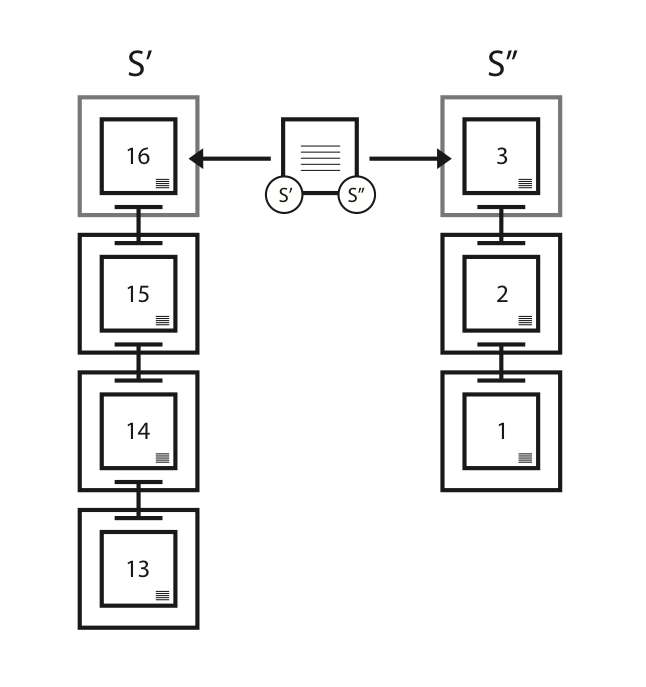
\includegraphics [width=\textwidth]{boundwitness}
\begin{center}\textbf{Figure 2.}  Record Logging Example Between Two Sentinels
\end{center}

\subsection{Origin Chains}

Specifically, each origin maintains its own ledger and signs it to make a Proof of Origin Chain. Once information on the Proof of Origin Chain has been shared, it is effectively permanent. This is because the fork that happens after the share ends the chain and makes all future data from the witness to be treated as if it was from a new witness. To generate a link in a Proof of Origin Chain, the origin generates a public/private key pair. It then signs both the previous and next blocks with the same pair after including the public key in both blocks. Immediately after the signature is made, the private key is deleted. With the immediate deletion of the private key, the risk of a key being stolen or reused is greatly minimized.

\Glspl{origin-chain} are the key to verifying that ledgers flowing into the \Gls{xyo-network} are valid. A unique ID for source of data is not practical since it can be forged. Private Key signing is not practical since most parts of the XYO Network are difficult or impossible to physically secure, thus the ability for a bad actor to steal a Private Key is too feasible. To solve this, XYO Network uses \Glspl{transient-key-chain}. The benefit of this is that it is impossible to falsify the chain of origin for data. However, once the chain is broken, it is broken forever and cannot be continued, rendering it an island.

Every time a \gls{heuristic} ledger is handed off in XYO Network, the receiver appends their own \Gls{proof-of-origin}, which makes the Proof of Origin chain bigger and generates a Proof of Origin Intersection. Proof of Origin Chains and Proof of Origin Intersections are the primary indicators used by \Glspl{diviner} to verify validity of ledgers. The equation for a Ledger Reputation is effectively what percent of the XYO Network was involved in making the Proof of Origin Ball associated with it. In theory, if 100 percent of the XYO Network records are linked with Proof of Origin and then fully analyzed, the odds of it being valid is 100 percent. If 0 percent of XYO Network records are available for analysis, then validity drops to 0 percent.

For added security, the Public Key for a Chain Link is not provided until the second entry for it is made available. This allows for the time interval between entries or other data to be added to the link.

\subsection {Origin Chain Score}
\Gls{origin-chain-score} is calculated as follows (default algorithm):

\begin{itemize}
\item PcL = \Gls{proof-of-origin} Chain Length
\item PcD = Proof of \Gls{origin-chain} Difficulty
\item Pc' Pc'' O = Proof of Origin Chain Overlap for Pc' and Pc''
\end{itemize}

\begin{equation*}\tag{1} \label{eq1}
Score = \prod_{i=0}^{i=n} \frac{PcL*PcD}{Pc' Pc'' O}
\end{equation*}

\subsection {Origin Tree}
An \Gls{origin-tree} is used to calculate the approximate validity of an answer. It uses the data gathered to generate an Ideal Tree, which is the tree that best fits that data for a given asserted answer. If Node \textit{N} is located at X,Y,Z,T location, the error across all the data in the set must hold a certain value. To compute this error, we would calculate the MIN, MAX, MEAN, MEDIAN, and AVERAGE DISTANCE FROM THE MEAN.

The asserted answer that has the highest: [Difficulty * (1 - percent error)], is the Best Answer. Using the Proof of Origin Tree, we can identify and prune impossible branches.

\subsection{Transient Key Chaining}

A series of data packets can be chained together by using temporary private keys to sign two successive packets. When the public key paired with the private key is included in the data packets, the receiver can verify that both packets were signed by the same private key. The data in the packet cannot be altered without breaking the signature, assuring that the signed packets were not altered by a third party, such as a Bridge or storage node.

\subsection {Link Depth}
At a minimum, a node generates a new public/private key pair for every link in the Proof of Origin Chain, which has a Link Depth of \texttt{1}. There may be \texttt{N} entries in the link table for a given \textit{Ledger Entry}, with each entry specifying the distance in the future when part two of the link will be added. No two links may have the same order of magnitude on a base 2 scale. For example, \textit{[1,3,7,12,39]} would be allowed, but \textit{[1,3,7,12,15]} would not.

The depth 1 link is created, used and deleted when the previous block is published. However, links of depth greater than 1 have their pair generated as the previous block is being signed, and the second signing does not happen until \textit{N} blocks later, after which the private key is deleted. For this reason, links of depth greater than 1 are always considered to be less secure than links of depth 1, but they can be used to improve performance and reduce data loss at the cost of that security.

\subsection {Fixed Order}
A key method for determining the sequence of ledgers is the order in which they were reported. Given that it is not possible for a device to change the order of any \Gls{proof-of-origin} signed ledger, an absolute order can be established by looking at all the Ledgers together.

\subsection {Second-to-Last Publishing}
A primary method for establishing \Gls{proof-of-origin} is the fact that a \Gls{sentinel} always reports its second to last block without reporting the last block. This allows the last block to have the signed link to its predecessor as evidence of the link.

\subsection {Empty Links}
To make a Proof of Origin Chain more secure, it is required that the chain is updated no more than once every ten seconds and no less than once every sixty minutes. In the case that no new data is available, an empty block will be added to the chain.

\subsection {Diagram}
As time travels from left to right (Figure 3.), the Proof of Origin Chain that is being built gets longer. At any given time, the producer of the chain will only provide to the caller the entries with darkened borders, waiting for the second signing of the entry before making it available. For example, in the 3rd column, only entry 2 and 1 will be returned as being part of the chain.

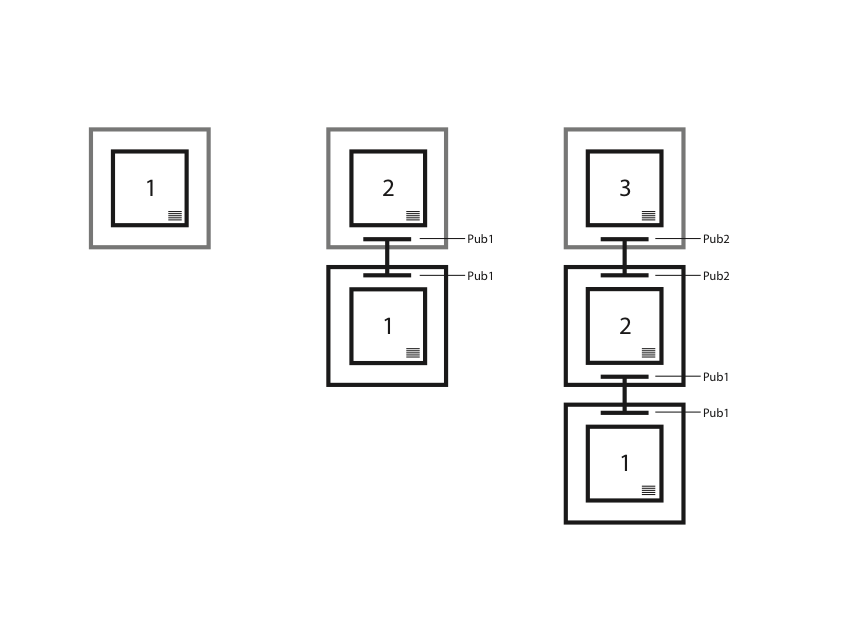
\includegraphics[width=\textwidth] {proofoforigin}
\begin{center}\textbf{Figure 3.}  Link inclusion example in a Proof of Origin Chain
\end{center}

\subsection {Summary}
\textbf{Given a series of data packets that are signed in sequential pairs with temporary private keys and include the paired public keys, it can be determined with absolute \gls{certainty} that the packets came from the same origin.}

\begin{center}
\line(1,0){50}
\end{center}

\section{Security Considerations}

\subsection{Fake Diviner Attack}

A set of digital signatures are sent to the XY Ethereum smart contract because the contract needs to verify the integrity of the Diviner that sent the answer. The contract can then verify the other Diviners that signed this signature within a high confidence interval. Without this, the relaying oracle would be the single source of failure and risk within the system.

\subsection{Sentinel DDoS Attacks}

Another important attack is Distributed Denial of Service among sentinel nodes in a particular region. An attacker could attempt to establish a large number of connections to sentinels in order to prevent them from relaying the correct information or relaying any information at all to the Bridges. We can circumvent this problem by requiring a small cryptographic puzzle to be solved by anyone attempting to connect to a sentinel. Since a query won't involve a very large number of connections to sentinels, this will not have a heavy bearing on the XYO relay system, and will require an attacker to spend a large amount of resources to successfully DDoS our network. At any given point in time, an Origin Chain can be verified by anyone as it is stored on the XYMainChain, ensuring that if a single entity along the chain was compromised, the accuracy of the query's answer (Origin Chain Score) will go to 0.

\begin{center}
\line(1,0){50}
\end{center}

\section {XYO Token Economy}

\Glspl{oracle} stand as a significant portion of the power and infrastructure needs for decentralized applications, with most of the focus revolving around the connectivity and aggregation of authoritative oracles. We believe that the need for a fully decentralized and trustless system of oracles is needed for decentralized applications to reach their maximum potential.

\subsection {XYO Network Cryptoeconomics}
 We use XYO to incentivize the desired behavior of providing accurate, reliable location \glspl{heuristic}. XYO Tokens can be thought of as``gas'' needed to interface with the real world in order to verify the XY-coordinate of a specified object.

The process works like this: A token holder queries the XYO Network with a query, (e.g. ``Where is my eCommerce order package with XYO Address \texttt{0x123456789}''). The query gets sent into a queue, where it waits to be processed and answered. A user can set their desired confidence level and XYO gas cost at query creation. The cost of a query (in XYO tokens) is determined by the amount of data required to provide an answer to the query and will depend on market dynamics.  The more data needed, the more expensive the query and higher the XYO Gas Price. Potential queries to the XYO Network can be very large and expensive. For instance, a trucking and logistics company could query the XYO Network to ask, \textit{``What is the location of every single car in our fleet?''}

Once the XYO Token holder queries the XYO Network and pays the requested gas, Diviners taking hold of the task call out to the relevant \Gls{archivist} to retrieve the pertinent data needed to answer the query. The data returned is derived from the \Glspl{bridge}, who originally gathered the data from the \Glspl{sentinel}. Sentinels are essentially devices or signals that verify the location of objects. These include devices like Bluetooth trackers, GPS trackers, geo-location tracking built into IoT devices, satellite tracking technology, QR-code scanners, RFID scanning and many others. XY Findables has pioneered and launched its consumer business, XY Find It, which has allowed it to test and process real-world location heuristics. All efforts of XY Find It have served to help significantly in designing the XYO Network Blockchain Protocol.

If the data provided by a Sentinel device (i.e. XY Find It Beacon) is used to answer a query, then all four Components involved in the transaction receive a part of the XYO Gas paid by the token holder: the Diviner (who searched for the answer), the Archiver (who stored the data), the Bridge (who transmitted the data) and the Sentinel (who recorded the location data)receive a part of the XYO Gas paid by the token holder. The distribution of the gas between the 4 components of the XYO Network always happens in the same proportion. Within each component, gas gets distributed evenly except for Diviners, who need to put in a lot more work than every other component.

\subsection{Rewards for Independence}

Location-gathering devices are the atomic blocks of the network, and a single device may act as one or more of these four components of the system. However, it would be rare, especially in a large XYO Network, that devices would be more than two of these components. Proof of Origin encompasses Furthermore, a blockchain ledger that has more independent Proof of Origin will hold higher regard, so there is a cryptoeconomic penalty for a device acting as multiple components.

\subsection{Rewards for Stationarity Integrity}

Sentinels in the XYO Network are assigned a stationarity coefficient for their quantity of movement throughout their lifecycle. The less a sentinel moves in a period of time, the more we can trust its data. Archivists keep track of these stationarity coefficients and they come into play when considering which sentinels to route queries to.

\subsection{Incentivizing Token Usage}
A system in which the holder is encouraged to \textit{not} use their tokens rather than transacting with their tokens creates a long-term problem for the underlying economy.  It creates an ecosystem with very scarce stores of value and triggers a natural impulse to invent reasons for \textit{not} using the coin instead of creating utility and liquidity. Lack of token liquidity is often ignored by token holders because the artificial scarcity created by reticent token-spending creates short-term spikes, but the question is: at what cost?

\textbf{The problem of most cryptoeconomic incentives centers on their focus. The focus is placed too strongly on the token miners, and not at all on the token users. The XYO Token to take both into account by defining the ideal-state and rewarding the market participants who hold in-memory accounts of the ideal-state and act upon reaching it.}.

In a XYO crypto-location mining pool (\textit{XYO Miners})  where the majority of XYO Miners are low quality, the entire pool of XYO Miners can vote to set the location-verification bar low; however as soon as more and more cheaper machines are introduced to the pool, with just as much (if not more power than the previous ones), the system votes to increase its Ideal State for the system. Thus the progression of the system lays in direct proportion with the advancements in computing technology of the world (not in computing technology of a few centralized mining pools with access to the most powerful computer machine manufacturers).

At different points in the token's economy, the user is rewarded with different token reward rates depending on the natural flow of the system as part of XYO's liquidity incentives. In a system where transactions are rampant, a user who preserves the token won't be missing out on transacting. However just as safety measures are put in place for preventing fraud amongst miner coming up with the wrong answers, by punishing them with XYO Token loss, so too will users be punished who are trying to game the system by transacting with other parties in a circular manner in hopes of gaming tokens (i.e. sending XYO back and forth between friends over and over to get rewarded in token rewards).


The miner is incentivized to not just provide accurate data, but also to know when to not provide data at all. The end user is rewarded to transact more when network liquidity is low, compared to when network liquidity is high.

Similar to how credit cards reward consumers for spending money, in this model the consumer receives rewards which are given up by XYO Miners who could have computed or verified the data, but elected not to for the health of the ecosystem. Essentially, the rich machines forfeit the reward they would have received and passed it on to the end-user transacting (as well as the second-best machine that took its place for not acting), in order to create a better token system. Thus proving that it has the best intent of the token ecosystem in mind.

\subsection {XYO Token Specifications}
\begin{itemize}
\item Smart contract platform: Ethereum
\item Contract Type: ERC-20
\item Token: XYO
\item Token Name: \Gls{xyo-network} Utility Token
\item Token Address: 0x55296f69f40ea6d20e478533c15a6b08b654e758
\item Total issuance: Finite and capped at the amount reached after the Token Main Sale
\item Amount issued during the main sale: Unlimited
\item Unsold and Unallocated tokens: Burned after the token sale event. No further XYO tokens will be generated after the Main Sale ends.
\end{itemize}

\begin{center}
\line(1,0){50}
\end{center}

%Use Cases Section
\section{XYO Network Use Cases}
The \Gls{xyo-network}'s usage  has vast applications that span a multitude of industries. Take for example an eCommerce Company that could offer its premium customers payment-upon-delivery services. To be able to offer this service, the eCommerce company would leverage the XYO Network and XY Platform (which uses XYO Tokens) to write a \gls{smart-contract} (i.e. on Ethereum's platform). The XYO Network could then track the location of the package being sent to the consumer along every single step of fulfillment; from the warehouse shelf to the the shipping courier, all the way into the consumer's house and every location in between. This could enable eCommerce retailers and websites to verify, in a trustless way, that the package not only appeared on the customer's doorstep, but also safely inside their home. Once the package has arrived in the customer's home (defined and verified by a specific XY-Coordinate), the shipment is considered complete and the payment to the vendor gets released. The eCommerce integration of the XYO Oracle Network thusly enables the ability to protect the merchant from fraud and ensure consumers only pay for goods that arrive in their home.

Consider an entirely different integration of the XYO Network with a hotel review site, whose current problem is that their reviews are often not trusted. Naturally, hotel owners are incentivized to improve their reviews at any cost. What if one could say with extremely high \gls{certainty} that someone was in San Diego, flew to a hotel in Bali and stayed there for two weeks, returned to San Diego, and then wrote a review about their hotel stay in Bali? The review would have a very high reputation, especially if it was written by a serial reviewer who has written many reviews with verified location data.

\begin{center}
\line(1,0){50}
\end{center}

\section {XYO Network Expansion}
We are fortunate to have a consumer business that has successfully built a real-world network with over one million (1,000,000) bluetooth and GPS devices in the world. Most location networks fail to reach this phase and get the critical mass necessary to building out an extensive network. However the Sentinel network we have created is only the starting point. The XYO Network is an open system that any operator of location devices can plug into the XYO Network and begin earning XYO Tokens.

To further grow its network, the \Gls{xyo-network} is engaging with businesses to expand its network of \Glspl{sentinel} beyond its own network of XY Find It beacons, which total to over 800,000 globally as of January 2018. A variety of devices can act as Sentinels. Generally, the greater the Sentinel cardinality in the XYO Network, the more reliable the network.

% TODO:
\section {Acknowledgements}

We thank Johnny Kolasinski and Christine Sako for their research and compilation of applicable use cases, and their work in auditing the white paper for formatting consistency. We also thank the following individuals for their comments and insight in reviewing our work: John Arana and Raul Jordan.

\clearpage

\printglossaries

%*******************************
%**** End Glossary Section *****
%*******************************

\end{document}
